\makeatletter
\def\input@path{{../}}
\makeatother
\documentclass[../master_thesis.tex]{subfiles}
\begin{document}
\chapter{Results}
\section{Description of Systems}
In order to test our implementation of the solvent effect as done in \cite{FossoTande:2013ka}
we will be comparing results with two sets of data, calculated data from Gaussian
computational chemistry software and test data from Chipman \cite{Chipman2002}.
The solute molecules in question are \ce{H_2O}, \ce{NO^+}, \ce{CN^-},
\ce{CH_3CONH_2} and \ce{Li^+}. The solvent is water with a dielectric constant
$\epsinf$ of $78.304$.

The first tests consisted of using only a single cavity for all the molecule and
increasing its radius from $3.6 a.u.$ to $5.0 a.u.$ by increments of $0.1 a.u.$.
This was done to all the solute molecules above, except for  \ce{CH_3CONH_2} which
was too large for these tests. This was done in Mrchem with relative precision of
$1.0e-5$ and a cavity boundary width of $\sigma = 0.2$. In Gaussian these tests were
ran using \ac{HF} method with coupled cluster basis sets (keyword cc-pVXZ where X
can be replaced by D, T, Q and 5) and increasing their completeness. These were
began as normal coupled cluster, then augmented and finally double augmented.

Then we tested atom centered intersecting spheres cavity (Here called \ac{ABC})
with radii equal to the Bondi radii of the atoms in the molecules \cite{doi:10.1021/j100785a001} scaled by $1.2$
\cite{Tomasi:1994wt}, which was done for all solutes (\ce{Li^+} was not necessary as it
is just a single atom). The \ac{ABC} test was performed a second time, increasing the radii by $0.2 a.u.$.
Both sets were ran in Mrchem and Gaussian, with the same specifications as mentioned above.

For the second sets of tests we had to compare our results with \cite{Chipman2002}.
In this we had to make sure our starting points were the same, which was a simple
issue with \ce{H_2O} and \ce{NO^+}, since these calculations were already ran in the previous set
of tests. Chipman uses cavities of radius $4.0 a.u.$ for all its solutes except
for \ce{CN^-} for which a radius of $12.0 a.u.$ is used. This means that two calculations
need to be done in this part, one for a single cavity of radius $12 a.u.$ for \ce{CN^-}
and one with a single cavity of radius $4.0 a.u.$ for \ce{CH_3CONH_2}. Two additional tests for
each were done, one where we increased and one where we decreased the radius by $0.2 a.u.$
for both solutes.

The reasoning behind using several radii in the tests is because of the amount of
charge that escapes the cavity. Since the cavity function we are using is analytical
instead of a boundary condition, we can't assume all the charge distribution
is contained within it. By varying the radii we can sample what radii in Mrchem
is best suited to represent radii in calculations in Gaussian or in \cite{Chipman2002}

\section{Data}
\subsection{\ac{ABC} tests}
The data tables containing all results can be found at the end of the chapter in section \ref{Datatables}, following
tales will show a small sample so the reader can make better understand the tables
in the appendixes.

The following table \ref{tab:rawwaterdata}  presents the data for the energy
calculations of \ce{H_2O} with the three first cavity radii as an example.
These are the total \ac{SCF} energy values.
The same type of tables were used for the rest of the
systems.
\begin{table}[htbp]
\caption{Total Energy Calculations example for Water in Water. Energy in Hartree and radii of the cavity in Bohr}
\begin{center}
\begin{tabular}{|l|r|r|r|r|}
\hline
Basis & $R =3.6$ & $R=3.7$ & $R=3.8$ & $\ldots$\\  \hline
Cc-pVDZ & -7.6039e+01 & -7.6038e+01 & -7.6036e+01 & $\ldots$\\ \hline
Cc-pVTZ & -7.6070e+01 & -7.6069e+01 & -7.6067e+01 & $\ldots$\\ \hline
Cc-pVQZ & -7.6078e+01 & -7.6076e+01 & -7.6075e+01 & $\ldots$\\ \hline
Cc-pV5Z & -7.6080e+01 & -7.6079e+01 & -7.6077e+01 & $\ldots$\\ \hline
Aug-cc-pVDZ & -7.6054e+01 & -7.6053e+01 & -7.6052e+01 & $\ldots$\\ \hline
Aug-cc-pVTZ & -7.6074e+01 & -7.6072e+01 & -7.6071e+01 & $\ldots$\\ \hline
Aug-cc-pVQZ & -7.6079e+01 & -7.6077e+01 & -7.6076e+01 & $\ldots$\\ \hline
Aug-cc-pV5Z & -7.6080e+01 & -7.6079e+01 & -7.6077e+01 & $\ldots$\\ \hline
daug-cc-pVDZ & -7.6055e+01 & -7.6053e+01 & -7.6052e+01 & $\ldots$\\ \hline
daug-cc-pVTZ & -7.6074e+01 & -7.6072e+01 & -7.6071e+01 & $\ldots$\\ \hline
daug-cc-pVQZ & -7.6079e+01 & -7.6077e+01 & -7.6076e+01 & $\ldots$\\ \hline
daug-cc-pV5Z & -7.6080e+01 & -7.6079e+01 & -7.6077e+01 & $\ldots$\\ \hline
mrchem & -7.6085E+01 & -7.6083E+01 & -7.6081E+01 & $\ldots$\\ \hline
\end{tabular}
\end{center}
\label{tab:rawwaterdata}
\end{table}

In order to get the Reaction field
energies $E_r$ one needs the gas state Energy $E_{vac}$ for a given
basis set and subtract it from the total solvent energy $E_{tot}$ calculated for
that basis set.
\begin{equation}
  E_r = E_{tot} - E_{vac}
\end{equation}
Examples for the first three radii for the results of the above operation can be
seen in table \ref{tab:Erwatdata}

\begin{table}[htbp]
\caption{Reaction Field Energy Calculations example for Water in Water. Energy in Hartree and radii of the cavity in Bohr}
\begin{center}
\begin{tabular}{|l|r|r|r|r|}
\hline
basis & 3.6 & 3.7 & 3.8 & $\ldots$\\ \hline
Cc-pVDZ & -1.2450E-02 & -1.0998E-02 & -9.7804E-03 & $\ldots$\\ \hline
Cc-pVTZ & -1.3097E-02 & -1.1545E-02 & -1.0243E-02 & $\ldots$\\ \hline
Cc-pVQZ & -1.3218E-02 & -1.1651E-02 & -1.0334E-02 & $\ldots$\\ \hline
Cc-pV5Z & -1.3284E-02 & -1.1713E-02 & -1.0393E-02 & $\ldots$\\ \hline
Aug-cc-pVDZ & -1.3190E-02 & -1.1634E-02 & -1.0328E-02 & $\ldots$\\ \hline
Aug-cc-pVTZ & -1.3238E-02 & -1.1670E-02 & -1.0353E-02 & $\ldots$\\ \hline
Aug-cc-pVQZ & -1.3221E-02 & -1.1655E-02 & -1.0338E-02 & $\ldots$\\ \hline
Aug-cc-pV5Z & -1.3223E-02 & -1.1655E-02 & -1.0337E-02 & $\ldots$\\ \hline
daug-cc-pVDZ & -1.3228E-02 & -1.1665E-02 & -1.0351E-02 & $\ldots$\\ \hline
daug-cc-pVTZ & -1.3243E-02 & -1.1675E-02 & -1.0357E-02 & $\ldots$\\ \hline
daug-cc-pVQZ & -1.3223E-02 & -1.1656E-02 & -1.0340E-02 & $\ldots$\\ \hline
daug-cc-pV5Z & -1.3224E-02 & -1.1655E-02 & -1.0337E-02 & $\ldots$\\ \hline
mrchem & -1.8036E-02 & -1.5494E-02 & -1.3437E-02 & $\ldots$\\ \hline
\end{tabular}
\end{center}
\label{tab:Erwatdata}
\end{table}

Following are figures \ref{fig:watEnergyplots},
% figures coming soon \ref{fig:nopEnergyplots} and \ref{fig:cyanEnergyplots}
show the energies of the mrchem calculations plotted
against the energies from the Gaussian calculation for water, \ce{NO^+}, and
\ce{CN^-} respectively.

\begin{figure}[h!]
  \centering
  \begin{subfigure}[b]{0.75\linewidth}
    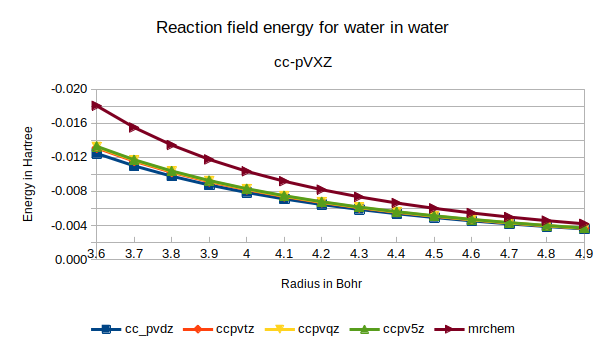
\includegraphics[width=\linewidth]{img/Erwat.png}
  \end{subfigure}
  \begin{subfigure}[b]{0.75\linewidth}
    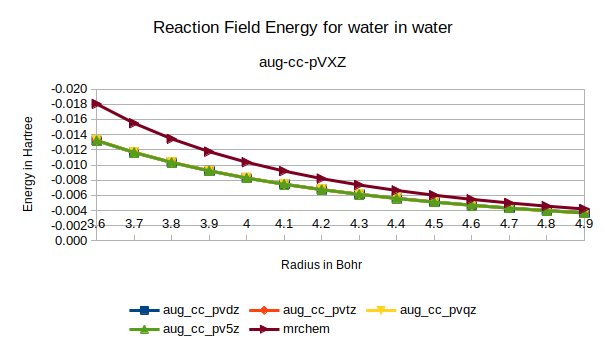
\includegraphics[width=\linewidth]{img/Eraugwat.png}
  \end{subfigure}
  \begin{subfigure}[b]{0.75\linewidth}
    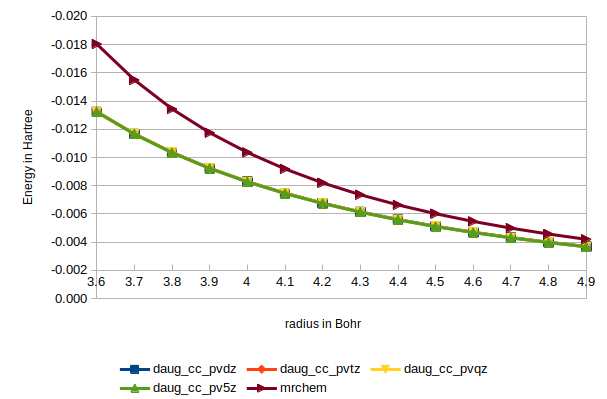
\includegraphics[width=\linewidth]{img/Erdaugwat.png}
  \end{subfigure}
  \caption{Reaction field energy of Water in a water solution, calculated with mrchem
  and with different basis sets in Gaussian}
  \label{fig:watEnergyplots}
\end{figure}

The Mrchem energy values $E_{Mrchem}$ for each radii were compared to the
corresponding values of each of the different basis set calculations in
Gaussian  $E_{Gaussian}^{basis}$ by finding the relative difference $d_r$
between them as
\begin{equation}\label{eq:reldiff}
  d_r = \frac{E_{Gaussian}^{basis} - E_{Mrchem}}{E_{Mrchem}}
\end{equation}
The operation above \ref{eq:reldiff} was applied to all the values for all the
substrate molecules, giving the following figures \ref{fig:watreldiff},
% figures coming soon \ref{fig:nopreldiff}, and \ref{fig:cyanreldiff}.

\begin{figure}[h!]
  \centering
  \begin{subfigure}[b]{0.75\linewidth}
    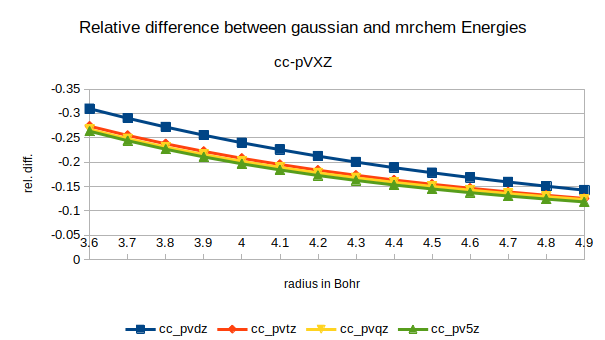
\includegraphics[width=\linewidth]{img/watreldiff.png}
  \end{subfigure}
  \begin{subfigure}[b]{0.75\linewidth}
    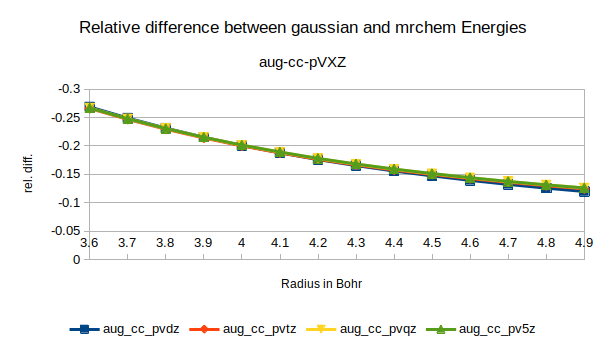
\includegraphics[width=\linewidth]{img/wataugreldiff.png}
  \end{subfigure}
  \begin{subfigure}[b]{0.75\linewidth}
    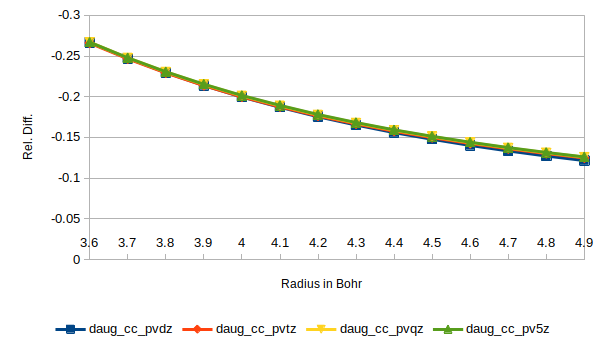
\includegraphics[width=\linewidth]{img/watdaugreldiff.png}
  \end{subfigure}
  \caption{Relative difference between the Reaction field energy of Water in a water solution calculated with mrchem
  and with different basis sets in Gaussian}
  \label{fig:watreldiff}
\end{figure}





\subsection{Chipman Comparison}

\section{Discussion}
\section{Conclusion}
\section{Areas of improvement/future development}

\section{Data tables}\label{Datatables}
\begin{sidewaystable}[htbp]

  \ttabbox{
  \resizebox{\textwidth}{!}{
  \begin{tabular}{|l|r|r|r|r|r|r|r|r|r|r|r|r|r|r|r|r|r|r|}
    \hline
    basis & \multicolumn{1}{l|}{vacuum E} & 3.6 & 3.7 & 3.8 & 3.9 & 4 & 4.1 & 4.2 & 4.3 & 4.4 & 4.5 & 4.6 & 4.7 & 4.8 & 4.9 & 5 & \multicolumn{1}{l|}{R = vdw*1.2} & \multicolumn{1}{l|}{R + 0.2} \\ \hline
    Cc-pVDZ & -7.6027E+01 & -7.6039E+01 & -7.6038E+01 & -7.6036E+01 & -7.6035E+01 & -7.6035E+01 & -7.6034E+01 & -7.6033E+01 & -7.6033E+01 & -7.6032E+01 & -7.6032E+01 & -7.6031E+01 & -7.6031E+01 & -7.6031E+01 & -7.6030E+01 & -7.6030E+01 & -7.6035E+01 & -7.6034E+01 \\ \hline
    Cc-pVTZ & -7.6057E+01 & -7.6070E+01 & -7.6069E+01 & -7.6067E+01 & -7.6066E+01 & -7.6065E+01 & -7.6064E+01 & -7.6064E+01 & -7.6063E+01 & -7.6063E+01 & -7.6062E+01 & -7.6062E+01 & -7.6061E+01 & -7.6061E+01 & -7.6061E+01 & -7.6060E+01 & -7.6066E+01 & -7.6064E+01 \\ \hline
    Cc-pVQZ & -7.6065E+01 & -7.6078E+01 & -7.6076E+01 & -7.6075E+01 & -7.6074E+01 & -7.6073E+01 & -7.6072E+01 & -7.6071E+01 & -7.6071E+01 & -7.6070E+01 & -7.6070E+01 & -7.6069E+01 & -7.6069E+01 & -7.6069E+01 & -7.6068E+01 & -7.6068E+01 & -7.6074E+01 & -7.6072E+01 \\ \hline
    Cc-pV5Z & -7.6067E+01 & -7.6080E+01 & -7.6079E+01 & -7.6077E+01 & -7.6076E+01 & -7.6075E+01 & -7.6074E+01 & -7.6074E+01 & -7.6073E+01 & -7.6073E+01 & -7.6072E+01 & -7.6072E+01 & -7.6071E+01 & -7.6071E+01 & -7.6071E+01 & -7.6070E+01 & -7.6076E+01 & -7.6074E+01 \\ \hline
    Aug-cc-pVDZ & -7.6041E+01 & -7.6054E+01 & -7.6053E+01 & -7.6052E+01 & -7.6050E+01 & -7.6050E+01 & -7.6049E+01 & -7.6048E+01 & -7.6047E+01 & -7.6047E+01 & -7.6046E+01 & -7.6046E+01 & -7.6046E+01 & -7.6045E+01 & -7.6045E+01 & -7.6045E+01 & -7.6050E+01 & -7.6049E+01 \\ \hline
    Aug-cc-pVTZ & -7.6060E+01 & -7.6074E+01 & -7.6072E+01 & -7.6071E+01 & -7.6070E+01 & -7.6069E+01 & -7.6068E+01 & -7.6067E+01 & -7.6067E+01 & -7.6066E+01 & -7.6066E+01 & -7.6065E+01 & -7.6065E+01 & -7.6064E+01 & -7.6064E+01 & -7.6064E+01 & -7.6069E+01 & -7.6068E+01 \\ \hline
    Aug-cc-pVQZ & -7.6066E+01 & -7.6079E+01 & -7.6077E+01 & -7.6076E+01 & -7.6075E+01 & -7.6074E+01 & -7.6073E+01 & -7.6073E+01 & -7.6072E+01 & -7.6071E+01 & -7.6071E+01 & -7.6070E+01 & -7.6070E+01 & -7.6070E+01 & -7.6069E+01 & -7.6069E+01 & -7.6075E+01 & -7.6073E+01 \\ \hline
    Aug-cc-pV5Z & -7.6067E+01 & -7.6080E+01 & -7.6079E+01 & -7.6077E+01 & -7.6076E+01 & -7.6075E+01 & -7.6075E+01 & -7.6074E+01 & -7.6073E+01 & -7.6073E+01 & -7.6072E+01 & -7.6072E+01 & -7.6071E+01 & -7.6071E+01 & -7.6071E+01 & -7.6071E+01 & -7.6076E+01 & -7.6075E+01 \\ \hline
    daug-cc-pVDZ & -7.6042E+01 & -7.6055E+01 & -7.6053E+01 & -7.6052E+01 & -7.6051E+01 & -7.6050E+01 & -7.6049E+01 & -7.6049E+01 & -7.6048E+01 & -7.6047E+01 & -7.6047E+01 & -7.6046E+01 & -7.6046E+01 & -7.6046E+01 & -7.6045E+01 & -7.6045E+01 & -7.6051E+01 & -7.6049E+01 \\ \hline
    daug-cc-pVTZ & -7.6061E+01 & -7.6074E+01 & -7.6072E+01 & -7.6071E+01 & -7.6070E+01 & -7.6069E+01 & -7.6068E+01 & -7.6067E+01 & -7.6067E+01 & -7.6066E+01 & -7.6066E+01 & -7.6065E+01 & -7.6065E+01 & -7.6064E+01 & -7.6064E+01 & -7.6064E+01 & -7.6070E+01 & -7.6068E+01 \\ \hline
    daug-cc-pVQZ & -7.6066E+01 & -7.6079E+01 & -7.6077E+01 & -7.6076E+01 & -7.6075E+01 & -7.6074E+01 & -7.6073E+01 & -7.6073E+01 & -7.6072E+01 & -7.6071E+01 & -7.6071E+01 & -7.6071E+01 & -7.6070E+01 & -7.6070E+01 & -7.6069E+01 & -7.6069E+01 & -7.6075E+01 & -7.6073E+01 \\ \hline
    daug-cc-pV5Z & -7.6067E+01 & -7.6080E+01 & -7.6079E+01 & -7.6077E+01 & -7.6076E+01 & -7.6075E+01 & -7.6075E+01 & -7.6074E+01 & -7.6073E+01 & -7.6073E+01 & -7.6072E+01 & -7.6072E+01 & -7.6071E+01 & -7.6071E+01 & -7.6071E+01 & -7.6071E+01 & -7.6076E+01 & -7.6075E+01 \\ \hline
    mrchem & -7.6067E+01 & -7.6085E+01 & -7.6083E+01 & -7.6081E+01 & -7.6079E+01 & -7.6078E+01 & -7.6076E+01 & -7.6075E+01 & -7.6075E+01 & -7.6074E+01 & -7.6073E+01 & -7.6073E+01 & -7.6072E+01 & -7.6072E+01 & -7.6071E+01 & -7.4670E+01 & -7.6078E+01 & -7.6076E+01 \\ \hline
    variational & -7.6067E+01 & -7.6247E+01 & -7.6160E+01 & -7.6090E+01 & -7.6034E+01 & -7.5989E+01 & -7.5955E+01 & -7.5928E+01 & -7.5908E+01 & -7.5894E+01 & -7.5884E+01 & -7.5878E+01 & -7.5875E+01 & -7.5874E+01 & -7.5875E+01 & -7.4566E+01 & -7.6387E+01 & -7.6205E+01 \\ \hline
  \end{tabular}}}{\caption{Total Energy of \ce{H_2O}. Radius in top row in Bohr and energies in Hartree}
  \label{tab:rawwatdata}}

\ttabbox{

  \resizebox{\textwidth}{!}{
  \begin{tabular}{|l|r|r|r|r|r|r|r|r|r|r|r|r|r|r|r|r|}
    \hline
    basis & \multicolumn{1}{l|}{vac} & 3.6 & 3.7 & 3.8 & 3.9 & 4 & 4.1 & 4.2 & 4.3 & 4.4 & 4.5 & 4.6 & 4.7 & 4.8 & 4.9 & 5 \\ \hline
    Cc-pVDZ & -1.2893E+02 & -1.2907E+02 & -1.2906E+02 & -1.2906E+02 & -1.2906E+02 & -1.2905E+02 & -1.2905E+02 & -1.2905E+02 & -1.2904E+02 & -1.2904E+02 & -1.2904E+02 & -1.2904E+02 & -1.2903E+02 & -1.2903E+02 & -1.2903E+02 & -1.2903E+02 \\ \hline
    Cc-pVTZ & -1.2897E+02 & -1.2911E+02 & -1.2910E+02 & -1.2910E+02 & -1.2910E+02 & -1.2909E+02 & -1.2909E+02 & -1.2909E+02 & -1.2908E+02 & -1.2908E+02 & -1.2908E+02 & -1.2907E+02 & -1.2907E+02 & -1.2907E+02 & -1.2907E+02 & -1.2907E+02 \\ \hline
    Cc-pVQZ & -1.2898E+02 & -1.2912E+02 & -1.2911E+02 & -1.2911E+02 & -1.2911E+02 & -1.2910E+02 & -1.2910E+02 & -1.2910E+02 & -1.2909E+02 & -1.2909E+02 & -1.2909E+02 & -1.2908E+02 & -1.2908E+02 & -1.2908E+02 & -1.2908E+02 & -1.2908E+02 \\ \hline
    Cc-pV5Z & -1.2898E+02 & -1.2912E+02 & -1.2912E+02 & -1.2911E+02 & -1.2911E+02 & -1.2910E+02 & -1.2910E+02 & -1.2910E+02 & -1.2909E+02 & -1.2909E+02 & -1.2909E+02 & -1.2909E+02 & -1.2908E+02 & -1.2908E+02 & -1.2908E+02 & -1.2908E+02 \\ \hline
    Aug-cc-pVDZ & -1.2894E+02 & -1.2908E+02 & -1.2907E+02 & -1.2907E+02 & -1.2906E+02 & -1.2906E+02 & -1.2906E+02 & -1.2905E+02 & -1.2905E+02 & -1.2905E+02 & -1.2905E+02 & -1.2904E+02 & -1.2904E+02 & -1.2904E+02 & -1.2904E+02 & -1.2903E+02 \\ \hline
    Aug-cc-pVTZ & -1.2897E+02 & -1.2911E+02 & -1.2910E+02 & -1.2910E+02 & -1.2910E+02 & -1.2909E+02 & -1.2909E+02 & -1.2909E+02 & -1.2908E+02 & -1.2908E+02 & -1.2908E+02 & -1.2908E+02 & -1.2907E+02 & -1.2907E+02 & -1.2907E+02 & -1.2907E+02 \\ \hline
    Aug-cc-pVQZ & -1.2898E+02 & -1.2912E+02 & -1.2911E+02 & -1.2911E+02 & -1.2911E+02 & -1.2910E+02 & -1.2910E+02 & -1.2910E+02 & -1.2909E+02 & -1.2909E+02 & -1.2909E+02 & -1.2909E+02 & -1.2908E+02 & -1.2908E+02 & -1.2908E+02 & -1.2908E+02 \\ \hline
    Aug-cc-pV5Z & -1.2898E+02 & -1.2912E+02 & -1.2912E+02 & -1.2911E+02 & -1.2911E+02 & -1.2910E+02 & -1.2910E+02 & -1.2910E+02 & -1.2909E+02 & -1.2909E+02 & -1.2909E+02 & -1.2909E+02 & -1.2908E+02 & -1.2908E+02 & -1.2908E+02 & -1.2908E+02 \\ \hline
    daug-cc-pVDZ & -1.2894E+02 & -1.2908E+02 & -1.2907E+02 & -1.2907E+02 & -1.2906E+02 & -1.2906E+02 & -1.2906E+02 & -1.2905E+02 & -1.2905E+02 & -1.2905E+02 & -1.2905E+02 & -1.2904E+02 & -1.2904E+02 & -1.2904E+02 & -1.2904E+02 & -1.2904E+02 \\ \hline
    daug-cc-pVTZ & -1.2897E+02 & -1.2911E+02 & -1.2910E+02 & -1.2910E+02 & -1.2910E+02 & -1.2909E+02 & -1.2909E+02 & -1.2909E+02 & -1.2908E+02 & -1.2908E+02 & -1.2908E+02 & -1.2908E+02 & -1.2907E+02 & -1.2907E+02 & -1.2907E+02 & -1.2907E+02 \\ \hline
    daug-cc-pVQZ & -1.2898E+02 & -1.2912E+02 & -1.2911E+02 & -1.2911E+02 & -1.2911E+02 & -1.2910E+02 & -1.2910E+02 & -1.2910E+02 & -1.2909E+02 & -1.2909E+02 & -1.2909E+02 & -1.2909E+02 & -1.2908E+02 & -1.2908E+02 & -1.2908E+02 & -1.2908E+02 \\ \hline
    daug-cc-pV5Z & -1.2898E+02 & -1.2912E+02 & -1.2912E+02 & -1.2911E+02 & -1.2911E+02 & -1.2910E+02 & -1.2910E+02 & -1.2910E+02 & -1.2909E+02 & -1.2909E+02 & -1.2909E+02 & -1.2909E+02 & -1.2908E+02 & -1.2908E+02 & -1.2908E+02 & -1.2908E+02 \\ \hline
    mrchem & -1.2898E+02 & -1.2931E+02 & -1.2924E+02 & -1.2920E+02 & -1.2917E+02 & -1.2915E+02 & -1.2566E+02 & \multicolumn{1}{l|}{N/A} & -1.2565E+02 & -1.2565E+02 & -1.2911E+02 & \multicolumn{1}{l|}{N/A} & -1.2564E+02 & -1.2909E+02 & -1.2909E+02 & -1.2909E+02 \\ \hline
    variational & -1.2898E+02 & -1.2794E+02 & -1.2781E+02 & -1.2789E+02 & -1.2808E+02 & -1.2830E+02 & -1.2566E+02 & \multicolumn{1}{l|}{N/A} & -1.2565E+02 & -1.2565E+02 & -1.2900E+02 & -1.2905E+02 & -1.2564E+02 & -1.2909E+02 & -1.2910E+02 & -1.2910E+02 \\ \hline
  \end{tabular}}}{\caption{Total Energy of \ce{NO^+}.  Radius in top row in Bohr and energies in Hartree}
  \label{tab:rawnopdata}}


\ttabbox{

\resizebox{\textwidth}{!}{
\begin{tabular}{|l|r|r|r|r|r|r|r|r|r|r|r|r|r|r|r|r|r|r|}
\hline
basis & \multicolumn{1}{l|}{vac} & 3.6 & 3.7 & 3.8 & 3.9 & 4 & 4.1 & 4.2 & 4.3 & 4.4 & 4.5 & 4.6 & 4.7 & 4.8 & 4.9 & 5 & \multicolumn{1}{l|}{vdw} & \multicolumn{1}{l|}{R + 0.2} \\ \hline
Cc-pVDZ & -7.6027E+01 & -9.2425E+01 & -9.2425E+01 & -9.2423E+01 & -9.2422E+01 & -9.2420E+01 & -9.2418E+01 & -9.2416E+01 & -9.2414E+01 & -9.2412E+01 & -9.2410E+01 & -9.2408E+01 & -9.2405E+01 & -9.2403E+01 & -9.2401E+01 & -9.2399E+01 & -9.2414E+01 & -9.2410E+01 \\ \hline
Cc-pVTZ & -7.6057E+01 & -9.2455E+01 & -9.2455E+01 & -9.2454E+01 & -9.2453E+01 & -9.2452E+01 & -9.2451E+01 & -9.2449E+01 & -9.2447E+01 & -9.2445E+01 & -9.2443E+01 & -9.2441E+01 & -9.2439E+01 & -9.2437E+01 & -9.2435E+01 & -9.2433E+01 & -9.2448E+01 & -9.2444E+01 \\ \hline
Cc-pVQZ & -7.6065E+01 & -9.2464E+01 & -9.2463E+01 & -9.2463E+01 & -9.2462E+01 & -9.2461E+01 & -9.2460E+01 & -9.2458E+01 & -9.2456E+01 & -9.2455E+01 & -9.2453E+01 & -9.2451E+01 & -9.2449E+01 & -9.2447E+01 & -9.2445E+01 & -9.2443E+01 & -9.2457E+01 & -9.2453E+01 \\ \hline
Cc-pV5Z & -7.6067E+01 & -9.2465E+01 & -9.2465E+01 & -9.2465E+01 & -9.2464E+01 & -9.2463E+01 & -9.2462E+01 & -9.2460E+01 & -9.2459E+01 & -9.2457E+01 & -9.2455E+01 & -9.2454E+01 & -9.2452E+01 & -9.2450E+01 & -9.2448E+01 & -9.2446E+01 & -9.2460E+01 & -9.2456E+01 \\ \hline
Aug-cc-pVDZ & -7.6041E+01 & -9.2441E+01 & -9.2441E+01 & -9.2440E+01 & -9.2439E+01 & -9.2438E+01 & -9.2437E+01 & -9.2436E+01 & -9.2434E+01 & -9.2433E+01 & -9.2431E+01 & -9.2429E+01 & -9.2427E+01 & -9.2426E+01 & -9.2424E+01 & -9.2422E+01 & -9.2435E+01 & -9.2432E+01 \\ \hline
Aug-cc-pVTZ & -7.6060E+01 & -9.2459E+01 & -9.2459E+01 & -9.2459E+01 & -9.2458E+01 & -9.2457E+01 & -9.2456E+01 & -9.2454E+01 & -9.2453E+01 & -9.2451E+01 & -9.2449E+01 & -9.2448E+01 & -9.2446E+01 & -9.2444E+01 & -9.2442E+01 & -9.2441E+01 & -9.2454E+01 & -9.2450E+01 \\ \hline
Aug-cc-pVQZ & -7.6066E+01 & -9.2465E+01 & -9.2465E+01 & -9.2464E+01 & -9.2463E+01 & -9.2462E+01 & -9.2461E+01 & -9.2460E+01 & -9.2458E+01 & -9.2456E+01 & -9.2455E+01 & -9.2453E+01 & -9.2451E+01 & -9.2449E+01 & -9.2448E+01 & -9.2446E+01 & -9.2459E+01 & -9.2455E+01 \\ \hline
Aug-cc-pV5Z & -7.6067E+01 & -9.2466E+01 & -9.2466E+01 & -9.2465E+01 & -9.2464E+01 & -9.2463E+01 & -9.2462E+01 & -9.2461E+01 & -9.2459E+01 & -9.2457E+01 & -9.2456E+01 & -9.2454E+01 & -9.2452E+01 & -9.2450E+01 & -9.2449E+01 & -9.2447E+01 & -9.2460E+01 & -9.2457E+01 \\ \hline
daug-cc-pVDZ & -7.6042E+01 & -9.2441E+01 & -9.2441E+01 & -9.2440E+01 & -9.2440E+01 & -9.2439E+01 & -9.2437E+01 & -9.2436E+01 & -9.2435E+01 & -9.2433E+01 & -9.2431E+01 & -9.2430E+01 & -9.2428E+01 & -9.2426E+01 & -9.2424E+01 & -9.2423E+01 & -9.2435E+01 & -9.2432E+01 \\ \hline
daug-cc-pVTZ & -7.6061E+01 & -9.2459E+01 & -9.2459E+01 & -9.2459E+01 & -9.2458E+01 & -9.2457E+01 & -9.2456E+01 & -9.2454E+01 & -9.2453E+01 & -9.2451E+01 & -9.2449E+01 & -9.2448E+01 & -9.2446E+01 & -9.2444E+01 & -9.2443E+01 & -9.2441E+01 & -9.2454E+01 & -9.2450E+01 \\ \hline
daug-cc-pVQZ & -7.6066E+01 & -9.2465E+01 & -9.2465E+01 & -9.2464E+01 & -9.2463E+01 & -9.2462E+01 & -9.2461E+01 & -9.2460E+01 & -9.2458E+01 & -9.2456E+01 & -9.2455E+01 & -9.2453E+01 & -9.2451E+01 & -9.2449E+01 & -9.2448E+01 & -9.2446E+01 & -9.2459E+01 & -9.2455E+01 \\ \hline
daug-cc-pV5Z & -7.6067E+01 & -9.2466E+01 & -9.2466E+01 & -9.2465E+01 & -9.2464E+01 & -9.2463E+01 & -9.2462E+01 & -9.2461E+01 & -9.2459E+01 & -9.2457E+01 & -9.2456E+01 & -9.2454E+01 & -9.2452E+01 & -9.2450E+01 & -9.2449E+01 & -9.2447E+01 & -9.2460E+01 & -9.2457E+01 \\ \hline
mrchem & -9.2349E+01 & -9.2472E+01 & -9.2471E+01 & -9.2470E+01 & -9.2469E+01 & -8.9965E+01 & -9.2466E+01 & \multicolumn{1}{l|}{N/A} & -9.2463E+01 & \multicolumn{1}{l|}{N/A} & -8.9954E+01 & -9.2458E+01 & \multicolumn{1}{l|}{N/A} & -9.2454E+01 & -8.9945E+01 & -9.2450E+01 & -9.2463E+01 & \multicolumn{1}{l|}{N/A} \\ \hline
variational & -9.2349E+01 & -9.7694E+01 & -9.7347E+01 & -9.6991E+01 & -9.6630E+01 & -9.6271E+01 & -9.5920E+01 & \multicolumn{1}{l|}{N/A} & -9.5263E+01 & \multicolumn{1}{l|}{N/A} & -9.4678E+01 & -9.4432E+01 & -9.4199E+01 & -9.3990E+01 & -9.3801E+01 & -9.3632E+01 & -9.5400E+01 & -9.4773E+01 \\ \hline
\end{tabular}}} {\caption{Total Energy of \ce{CN^-}.  Radius in top row in Bohr and energies in Hartree}
\label{tab:rawcyandata}}
\end{sidewaystable}


\begin{acronym}
\acro{AUS}[\href{https://www.sigma2.no/content/advanced-user-support}{AUS}]{Numerical Methods in Quantum Chemistry}
\acro{BO}{Born-Oppenheimer}
\acro{CTCC}[\href{http://www.ctcc.no}{CTCC}]{Centre for Theoretical and Computational Chemistry}
\acro{DC}{Dielectric Continuum}
\acro{DFT}{Density Functional Theory}
\acro{EFP}{Effective Fragment Potential}
\acro{EU}{European Union}
\acro{HF}{Hartree-Fock}
\acro{Hylleraas}[\href{https://www.mn.uio.no/hylleraas/english/}{Hylleraas}]{Hylleraas
  Centre for Quantum Molecular Sciences}
\acro{HPC}{High Performance Computing}
\acro{KTH}{Royal Institute of Technology}
\acro{LDA}{Local Density Approximation}
\acro{MCD}{Magnetic Circular Dichroism}
\acro{MCSCF}{Multiconfiguration Self Consistent Field}
\acro{MM}{Molecular Mechanics}
\acro{MW}{Multiwavelet}
\acro{NFR}{Norwegian Research Council}
\acro{NMQC}[\href{http://www.ctcc.no/events/conferences/2015/numeric-conference/}{NMQC}]{Numerical Methods in Quantum Chemistry}
\acro{NOTUR}[\href{https://www.notur.no/}{NOTUR}]{Norwegian Metacenter for Computational Science}
\acro{PCM}{Polarizable Continuum Model}
\acro{PI}{Primcipal Investigator}
\acro{QC}{Quantum Chemistry}
\acro{QM}{Quantum Mechanics}
\acro{QM/MM}{Quantum Mechanics/Molecular Mechanics}
\acro{ROA}{Raman Optical Activity}
\acro{SC}{semiconductor}
\acro{SCF}{Self Consistent Field}
\acro{SHG}{Second Harmonic Genertation}
\acro{STSM}{Short-term scientific mission}
\acro{TPA}{Two-Photon Absorption}
\acro{WP}{Work Package}
\acro{CBS}{Complete Basis Set}
\acro{TCG}{Theoretical Chemistry Group}
\acro{vdW}{van der Waals}
\acro{SE}{Schrödinger Equation}
\acro{PES}{Potential Energy Surface}
\acro{LCAO}{Linear Combination of Atomic Orbitals}
\acro{MRA}{Multi-Resolution Analysis}
\acro{NS}{Nonstandard}
\end{acronym}

\biblio
\end{document}
